\section{Справочные сведения}\label{sec:general_information}
	\subsection{Общие сведения о походе}\label{subsec:general_information}
		\begin{longtable}{|>{\centering\arraybackslash} m{6.1cm}|>{\centering\arraybackslash} m{10cm}|} \hline
			Район похода														&	Российская Федерация, Кавказ (Безенги,~Приэльбрусье)						\\ \hline
			Вид туризма															&	Горный																		\\ \hline
			Категория сложности похода											&	Третья																		\\ \hline
			Проводящая организация												&	Горный турклуб МГУ, г.~Москва												\\ \hline
			Руководитель														&	Чашникова Анастасия Алекссандровна 											\\ \hline
			Контакты руководителя												&	тел.~+7(950)~816-39-44 e-mail:~chashni98@gmail.com 							\\ \hline
			Сроки активной части похода полные \newline (от Москвы до Москвы)	&	с 30 июня по 18 июля 2024 года \textit{(с~28~июня~по~20~июля~2024~года)}	\\ \hline
			Протяженность маршрута (по карте)									&	158.1\,км (163.6\,км с учётом радиальных выходов для части группы)			\\ \hline
			Длина маршрута с учётом $k = 1.1$									&	180\,км (из них в зачёт~-- 159.4\,км)										\\ \hline
			Продолжительность активной части									&	19 дней																		\\ \hline
			Суммарный набор/сброс, м											&	+13200/-13530																\\ \hline
			Максимальная высота													&	4370\,м (гребень в.~Башхауз)														\\ \hline
			Максимальная высота ночёвки											&	4185\,м (пер.~Тютю Зап.)													\\ \hline
		\end{longtable}\fxnote{Поправить километраж}
	
	
	\subsection{Запланированная нитка маршрута}\label{subsec:planned_route}
		\renewcommand{\bfdefault}{bx}
		\textit{
			Т/б~Уштулу~"---
			\fxnote{Поправить тире! не видны на нормальном масштабе!}
			\hyperref[subsec:main_obstacles]{пер.~Штулу + п.~Штулу (1А, рад.)}~"---
			д.р.~Карасу~"---
			приют Уштулу~"---
			д.р.~Черек Балкарский~"---
			д.р.~Тютюнсу~"---
			\hyperref[subsec:main_obstacles]{пер.~Туристов Грузии + пер.~Ашинова (1Б)}~"---
			лед.~Крумкол~"---
			\hyperref[subsec:main_obstacles]{пер.~Спартак + п.~Башхауз + пер.~МВТУ (2А)}~"---
			а/л~Безенги~"---
			\hyperref[subsec:main_obstacles]{пер.~Столбовой (2А)}~"---
			\hyperref[subsec:main_obstacles]{пер.~Тютюргу (1Б)}~"---
			\hyperref[subsec:main_obstacles]{пер.~Шаурту + п. МВТУ (2А)}~"---
			лед.~Шаурту~"---
			д.р.~Тютюргу~"---
			д.р.~Гара-Аузу-Су~"---
			д.р.~Башиль-Аузу-Су~"---
			т/б Башиль~"---
			д/р~Джайлык-Су~"---
			лед.~Джайлык~"---
			\hyperref[subsec:main_obstacles]{пер.~Кенчат + п.~Кенчатбаши + пер.~Килар (2А)}~"---
			лед.~Кенчат Западный~"---
			ночевки Тютю нижние~"---
			\hyperref[subsec:main_obstacles]{пер.~Тютю Зап. + п.~Тютюбаши 2-ая Зап. + пер.~Куллумкол + пер.~Шогенцукова (2А)}~"---
			д/р~Куллумкол-Су~"---
			а/л~Джайлык~"---
			Верхний Баксан.
			}\fxnote{Поправить ссылки!}
	
	\subsection{Пройденная нитка маршрута}\label{subsec:real_route}
		\textit{
			Т/б~Уштулу~"---
			\hyperref[subsec:main_obstacles]{пер.~Штулу + п.~Штулу (1А, рад.)}~"---
			д.р.~Карасу~"---
			приют Уштулу~"---
			д.р.~Черек Балкарский~"---
			д.р.~Тютюнсу~"---
			\hyperref[subsec:main_obstacles]{пер.~Туристов Грузии + пер.~Ашинова (1Б)}~"---
			лед.~Крумкол~"---
			\hyperref[subsec:main_obstacles]{пер.~Спартак + п.~Башхауз + пер.~МВТУ (2А)}~"---
			а/л~Безенги~"---
			\hyperref[subsec:main_obstacles]{пер.~Столбовой (2А)}~"---
			\hyperref[subsec:main_obstacles]{пер.~Тютюргу (1Б)}~"---
			\hyperref[subsec:main_obstacles]{пер.~Шаурту (2А)}~"---
			лед.~Шаурту~"---
			д.р.~Тютюргу~"---
			д.р.~Гара-Аузу-Су~"---
			д.р.~Башиль-Аузу-Су~"---
			т/б Башиль~"---
			д/р~Джайлык-Су~"---
			лед.~Джайлык~"---
			\hyperref[subsec:main_obstacles]{пер.~Надежда (1Б, п/п) + пер.~Кенчат + п.~Кенчатбаши (2А, рад.)}~"---
			\hyperref[subsec:main_obstacles]{пер.~Килар (1Б)}~"---
			лед.~Кенчат Западный~"---
			ночевки Тютю нижние~"---
			\hyperref[subsec:main_obstacles]{пер.~Тютю Зап. + п.~Тютюбаши 2-ая Зап. + пер.~Куллумкол + пер.~Шогенцукова (2А)}~"---
			д/р~Куллумкол-Су~"---
			а/л~Джайлык~"---
			Верхний Баксан.
			}\fxnote{Поправить ссылки!}
		\renewcommand{\bfdefault}{b}

		Маршрут пройден с изменениями, подробнее см. \ref{subsec:changes_of_way}.

	
	\subsection{Определяющие препятствия}\label{subsec:main_obstacles}
		\begin{longtable}{|>{\centering\arraybackslash}m{3.5cm}|>{\centering\arraybackslash}m{1.0cm}|>{\centering\arraybackslash}m{1.5cm}|>{\raggedright\arraybackslash}m{9.6cm}|>{\centering\arraybackslash}m{1.2cm}|} \hline
			Препятствие																																			&	К. т.	&	Высота				&	Краткое описание	&	ЧХВ	\\ \hline
			\hyperref[subsec:main_obstacles]{\begin{small}Пер.~Штулу~+ п.~Штулу\end{small}}														\newline\textit{радиально с запада}		&	1А		&	3570				&	\begin{small}Подъем на перевал Штулу - зямлянисто-травяной склон до $25^\circ$, короткие участки снежников до $15^\circ$. Путь от перевала до вершины проходит по сланцевой осыпи крутизной до $25^\circ$, также встречаются короткие участки пологих снежников.\end{small} &		\\ \hline
			\hyperref[subsec:main_obstacles]{\begin{small}Пер.~Туристов Грузии~+ пер.~Ашинова\end{small}}										\newline\textit{с севера на юг}			&	1Б		&	3640 3720			&		\begin{small}Подход по долине реки Тютюнсу под перевал Туристов Грузии трудоемок, большая его часть проходит по заросшей тропе. Встречаются участки заросших кустарниками каменистых склонов на прижимах реки, участки высокой тропы, заросли низкорослых деревьев. Подъем на перевал Туристов Грузии проходит по снежному склону до $25^\circ$ и не требует движения в кошках или подстраховку ледорубом. Есть очень короткие участки, на которых в менее снежное время года и в более ясную погоду есть вероятность схода камней. Седловина перевала широкая, снежно-осыпная, здесь вполне можно разбить лагерь. Спуск осуществляем в связках по леднику до $20^\circ$, преимущественно ледник закрытый. Подъем на перевал Ашинова проходит по снежному склону крутизной до $30^\circ$, движемся с самостраховкой ледорубом. Выкаты довольно пологие и безопасные. Седловина перевала очень широкая, мелкоосыпная, с нее открываются прекрасные виды на ГКХ, в котором доминируют отдельно стоящая Айлама и Шхара, с которой начинается Безенгийская стена. С другой стороны отлично виден массив Суганского хребта. Спуск проходит по мелколифтовой осыпи, несколько раз пересекаем участки подмерзших с ночи снежников до $25^\circ$, движемся в кошках с самостраховкой ледорубом. \end{small}&	\\ \hline
			\hyperref[subsec:main_obstacles]{\begin{small}Пер.~Спартак~+ п.~Башхауз~+ пер.~МВТУ\end{small}}										\newline\textit{с севера на юг}			&	2А		&	4090 4410 4215		&						&		\\ \hline
			\hyperref[subsec:main_obstacles]{\begin{small}Пер.~Столбовой\end{small}}															\newline\textit{с востока на запад}		&	2А		&	3690				&						&		\\ \hline
			\hyperref[subsec:main_obstacles]{\begin{small}Пер.~Тютюргу\end{small}}																\newline\textit{с севера на юг}			&	1Б		&	3835				&						&		\\ \hline
			\hyperref[subsec:main_obstacles]{\begin{small}Пер.~Шаурту\end{small}}																\newline\textit{с севера на юг}			&	2А		&	4085				&						&		\\ \hline
			\hyperref[subsec:main_obstacles]{\begin{small}Пер.~Кенчат~+ п.~Кенчатбаши\end{small}}												\newline\textit{радиально с востока}	&	2А		&	3905 4090			&						&		\\ \hline
			\hyperref[subsec:main_obstacles]{\begin{small}Пер.~Килар\end{small}}																\newline\textit{с востока на запад}		&	1Б		&	3885				&						&		\\ \hline
			\hyperref[subsec:main_obstacles]{\begin{small}Пер.~Тютю~Зап.~+ п.~Тютюбаши 2~Зап.~+ пер.~Куллумкол~+ пер.~Шогенцукова\end{small}}	\newline\textit{с севера на юг}			&	2А		&	4185 4300 3915 3590	&						&		\\ \hline
		\end{longtable}\fxnote{Доделать таблицу}
		

	\subsection{Состав группы}\label{subsec:group_composition}
		\begin{longtable}{|>{\centering\arraybackslash} m{3.5cm}|>{\centering\arraybackslash} m{3.6cm}|>{\centering\arraybackslash} m{3.5cm}|>{\centering\arraybackslash} m{2.5cm}|>{\centering\arraybackslash} m{2.5cm}|}\hline
			Фотография																																	&	ФИО										&	Должность					&	Год рождения	&	Опыт		\\ \hline
			\raisebox{-0.05\height}{\rule{0pt}{155pt}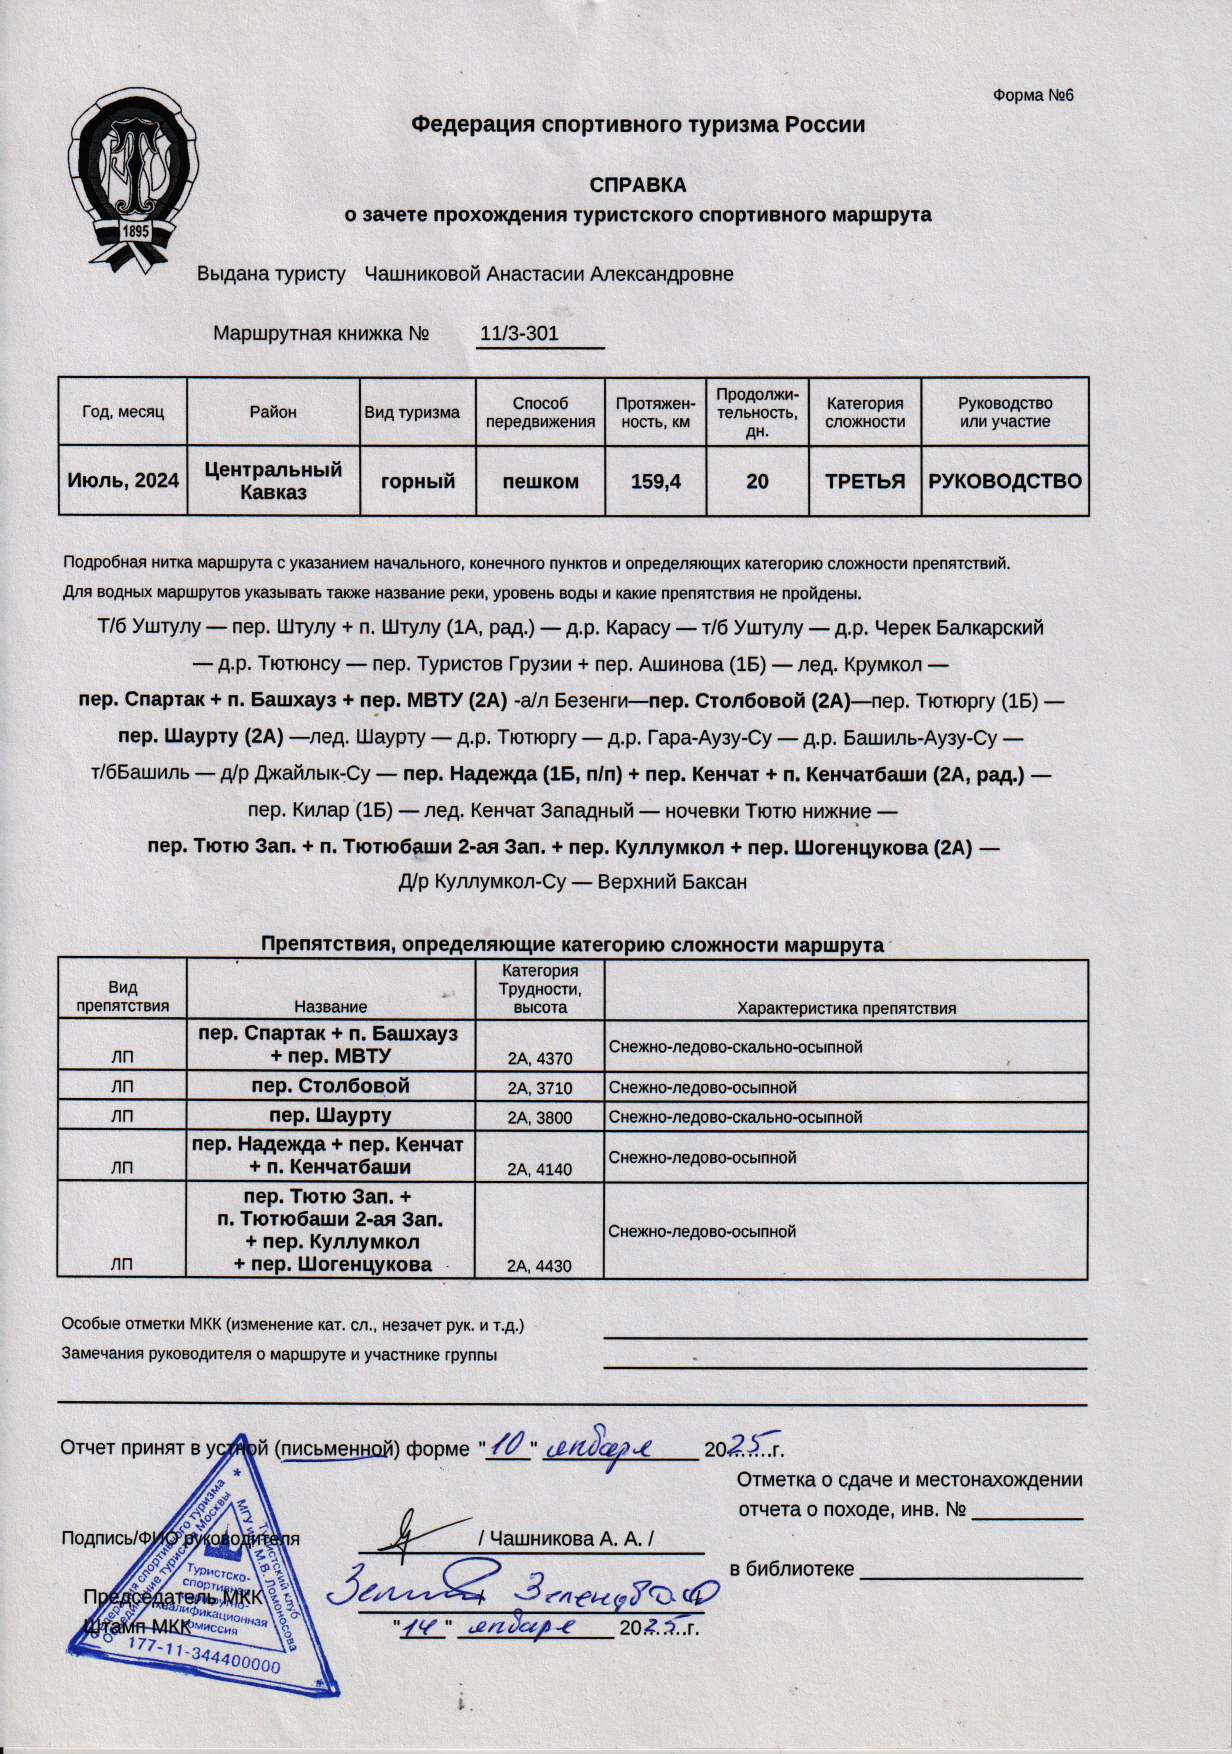
\includegraphics[width=3.5cm]{Pictures/Chapter1/Nastya.png}\raisebox{-1\height}{\rule{0pt}{5pt}}}	&	Чашникова Анастасия Алекссандровна		&	Руководитель				&	1998			&	4ГУ, 2ГР	\\ \hline
			\raisebox{-0.05\height}{\rule{0pt}{155pt}\includegraphics[width=3.5cm]{Pictures/Chapter1/Dima.png  }\raisebox{-1\height}{\rule{0pt}{5pt}}}	&	Коротков Дмитрий Юрьевич				&	Реммастер					&	2001			&	3ГУ, 1ГР	\\ \hline
			\raisebox{-0.05\height}{\rule{0pt}{155pt}\includegraphics[width=3.5cm]{Pictures/Chapter1/Dasha.png }\raisebox{-1\height}{\rule{0pt}{5pt}}}	&	Короткова Дарья Алексеевна				&	Завпит						&	2002			&	2ГУ			\\ \hline
			\raisebox{-0.05\height}{\rule{0pt}{155pt}\includegraphics[width=3.5cm]{Pictures/Chapter1/Katya.png }\raisebox{-1\height}{\rule{0pt}{5pt}}}	&	Мерчи-Байрамова Екатерина Вячеславовна	&	Логист						&	2002			&	2ГУ			\\ \hline
			\raisebox{-0.05\height}{\rule{0pt}{155pt}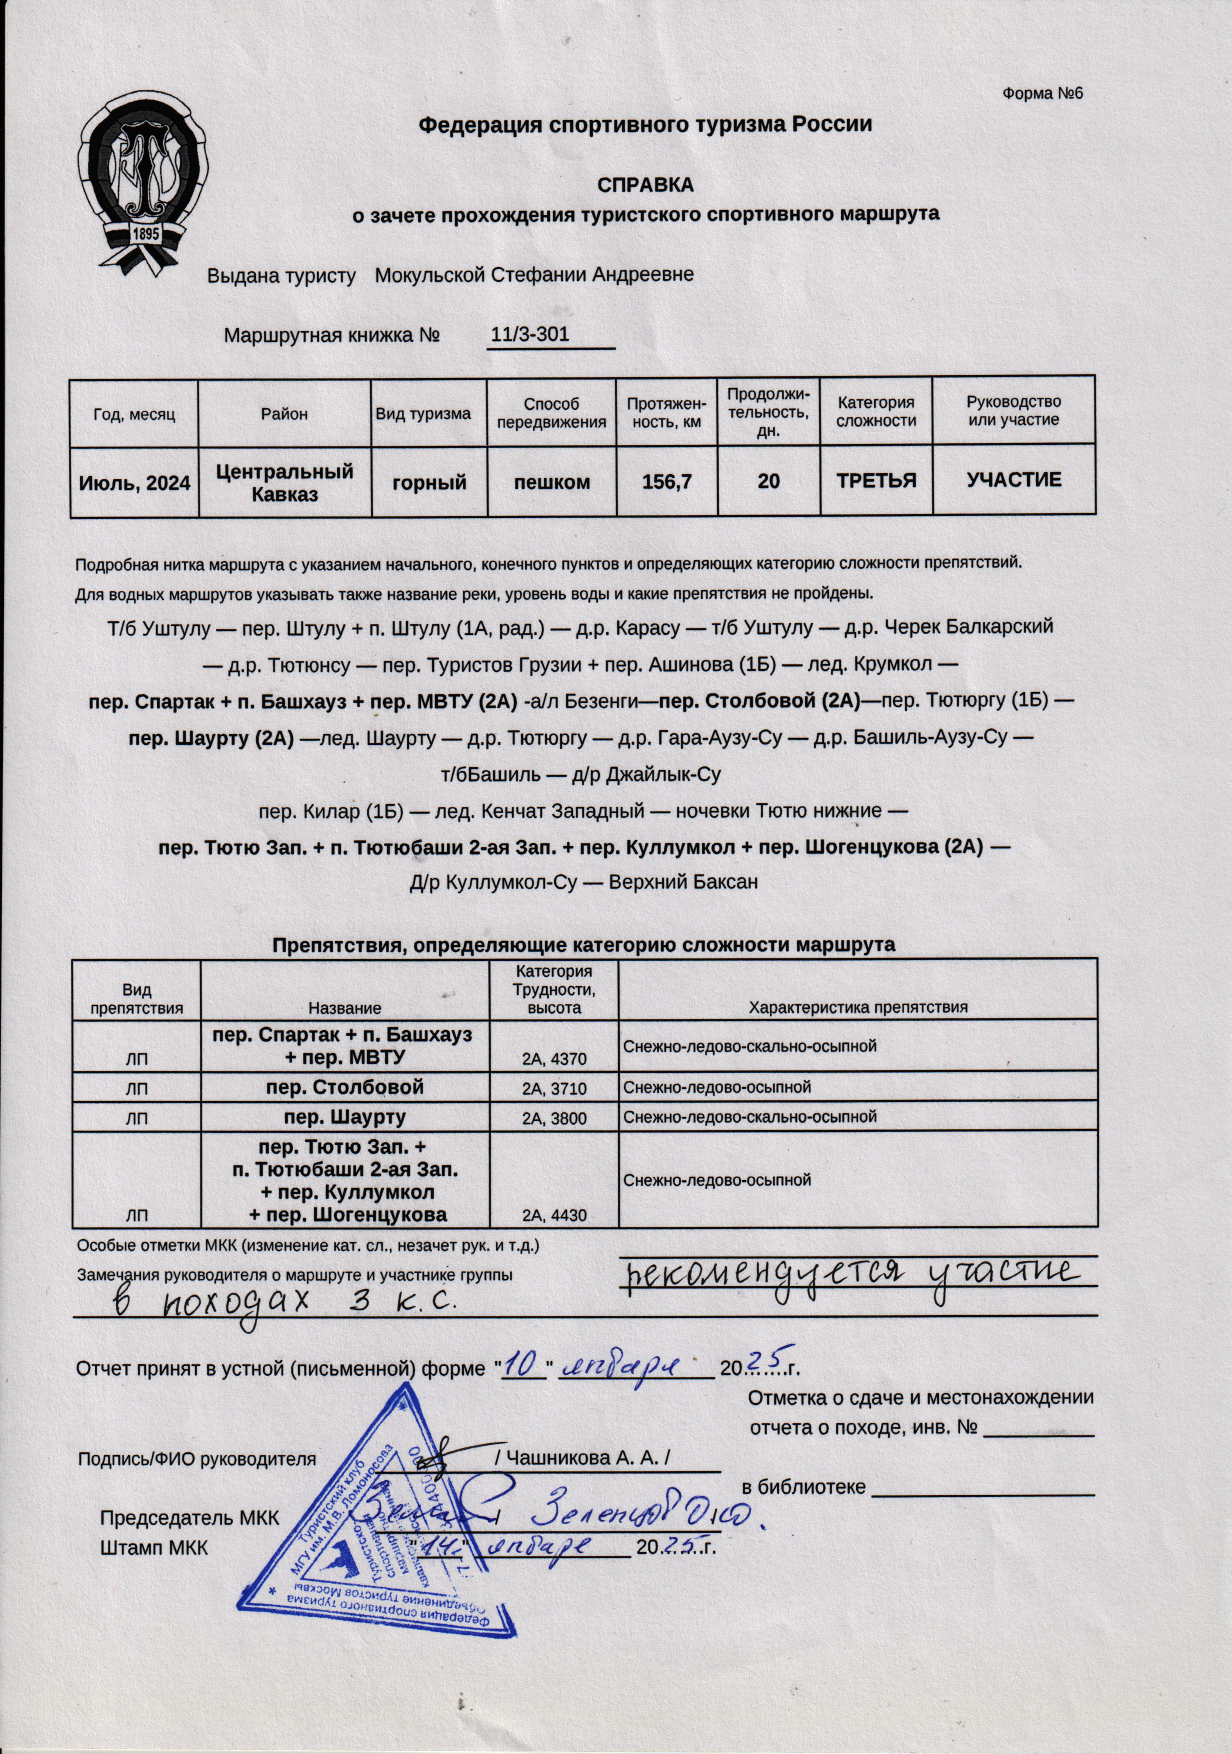
\includegraphics[width=3.5cm]{Pictures/Chapter1/Stepha.png}\raisebox{-1\height}{\rule{0pt}{5pt}}}	&	Мокульская Стефания Андреевна			&	Медик, фотограф				&	1997			&	2ГУ			\\ \hline
			\raisebox{-0.05\height}{\rule{0pt}{155pt}\includegraphics[width=3.5cm]{Pictures/Chapter1/Lesha.png }\raisebox{-1\height}{\rule{0pt}{5pt}}} 	&	Ткачёв Алексей Владимирович				&	Штурман						&	1988			&	2ГУ			\\ \hline
			\raisebox{-0.05\height}{\rule{0pt}{155pt}\includegraphics[width=3.5cm]{Pictures/Chapter1/Yura.png  }\raisebox{-1\height}{\rule{0pt}{5pt}}}	&	Цимбалов Юрий Александрович				&	Снаряженец, хронометрист	&	1989			&	4ГУ			\\ \hline
		\end{longtable}\fxnote{Найти нормальные фотки}

		Поход пройден группой в полном составе. Коротков Дмитрий и Короткова Дарья не участвовали в радиальном выходе на
		вер.~Штулу-Тау (дошли до высоты 3400\,м). Коротков Дмитрий, Короткова Дарья, Мокульская Стефания не участвовали
		в радиальном выходе на пер.~Надежда + пер.~Кенчат + вер.~Кенчатбаши.
		
